\section*{Profilo  di Caterina}

\subsection*{Neuroticismo}
\begin{itemize}
    \item \textbf{Ansia}: Alta \\
    Caterina tende a preoccuparsi facilmente, soprattutto riguardo alle sue prestazioni e al modo in cui gli altri la percepiscono. Fatica a gestire l'incertezza.
    
    \item \textbf{Irritabilità}: Moderata \\
    Non perde la calma facilmente, ma può diventare irritabile in situazioni di stress prolungato.
    
    \item \textbf{Depressività}: Moderata \\
    Ha momenti di insicurezza che possono abbassare il suo umore, ma non cade in stati depressivi gravi.
    
    \item \textbf{Autosufficienza}: Bassa \\
    Spesso si sente insicura riguardo alle proprie capacità e cerca approvazione esterna.
    
    \item \textbf{Vulnerabilità}: Alta \\
    In situazioni di stress elevato, Caterina può sentirsi sopraffatta e reagire con difficoltà.
\end{itemize}

\subsection*{Estroversione}
\begin{itemize}
    \item \textbf{Calore umano}: Alta \\
    Caterina si mostra accogliente e cerca connessioni profonde con chi le sta vicino.
    
    \item \textbf{Socievolezza}: Moderata \\
    Apprezza la compagnia degli altri, ma si sente più a suo agio con persone di fiducia.
    
    \item \textbf{Assertività}: Bassa \\
    Ha difficoltà a esprimere con decisione le proprie opinioni, soprattutto in contesti competitivi.
    
    \item \textbf{Vitalità}: Moderata \\
    È energica, ma solo in situazioni in cui si sente completamente a suo agio.
    
    \item \textbf{Ricerca di emozioni}: Bassa \\
    Non cerca emozioni forti o esperienze nuove, preferendo situazioni prevedibili.
    
    \item \textbf{Allegria}: Moderata \\
    Può essere gioiosa, ma il suo stato d'animo è spesso condizionato dalle sue insicurezze.
\end{itemize}

\subsection*{Apertura all’Esperienza}
\begin{itemize}
    \item \textbf{Immaginazione}: Alta \\
    Caterina ha una mente creativa, spesso alimentata dai suoi sogni e pensieri.
    
    \item \textbf{Interesse per l’arte}: Moderato \\
    Apprezza l’arte per le emozioni che suscita, più che per aspetti tecnici.
    
    \item \textbf{Sensibilità alle emozioni}: Alta \\
    È profondamente in contatto con le proprie emozioni e quelle degli altri.
    
    \item \textbf{Flessibilità mentale}: Moderata \\
    Aperta a nuove idee, ma ha bisogno di tempo per adattarsi a cambiamenti significativi.
    
    \item \textbf{Curiosità intellettuale}: Moderata \\
    Ama imparare, ma tende a sottovalutare le proprie capacità.
    
    \item \textbf{Ricerca di varietà}: Bassa \\
    Predilige routine e stabilità.
\end{itemize}

\subsection*{Amicalità}
\begin{itemize}
    \item \textbf{Fiducia negli altri}: Alta \\
    Caterina tende a vedere il meglio nelle persone, anche quando potrebbe essere più cauta.
    
    \item \textbf{Altruismo}: Alta \\
    È molto disponibile e disposta ad aiutare, spesso trascurando se stessa.
    
    \item \textbf{Disponibilità alla cooperazione}: Alta \\
    Si sforza di mantenere relazioni armoniose, evitando conflitti.
    
    \item \textbf{Modestia}: Alta \\
    Tende a sminuire le proprie capacità, a volte in modo eccessivo.
    
    \item \textbf{Empatia}: Alta \\
    Si identifica facilmente con le emozioni altrui e si preoccupa del loro benessere.
\end{itemize}

\subsection*{Coscienziosità}
\begin{itemize}
    \item \textbf{Competenza}: Moderata \\
    È competente, ma il suo bisogno di approvazione la limita.
    
    \item \textbf{Ordine}: Alta \\
    Organizzata e precisa, talvolta rigida nel seguire piani prestabiliti.
    
    \item \textbf{Duttilità}: Moderata \\
    È diligente, ma tende a procrastinare quando si sente sopraffatta.
    
    \item \textbf{Obiettivi personali}: Moderati \\
    Ambiziosa, ma spesso dubita di poter raggiungere i suoi obiettivi.
    
    \item \textbf{Autodisciplina}: Moderata \\
    Fatica a mantenere la concentrazione se non si sente motivata o sicura.
    
    \item \textbf{Prudenza}: Alta \\
    Riflette molto prima di agire, a volte fino a paralizzarsi nelle decisioni.
\end{itemize}

\newpage

\section*{Profilo di Laura}

\textbf{Neuroticismo}:
\begin{itemize}
    \item \textbf{Ansia}: Moderata. Tende a preoccuparsi in situazioni nuove o complesse, ma riesce a mantenere la calma di fronte a sfide tecniche.
    \item \textbf{Irritabilità}: Bassa. Laura è generalmente paziente e raramente si arrabbia, ma può sentirsi frustrata quando non riesce a raggiungere un obiettivo.
    \item \textbf{Depressione}: Bassa. Ha un atteggiamento positivo e si concentra su soluzioni piuttosto che sui problemi.
    \item \textbf{Autoconsapevolezza}: Alta. È consapevole delle proprie emozioni e tende a riflettere profondamente su di esse.
    \item \textbf{Impulsività}: Bassa. Prende decisioni in modo ponderato e raramente si lascia guidare dalle emozioni.
    \item \textbf{Vulnerabilità}: Moderata. Non si espone facilmente, ma sotto pressione può sentire il peso delle aspettative.
\end{itemize}

\textbf{Estroversione}:
\begin{itemize}
    \item \textbf{Calore umano}: Moderato. Ha pochi amici fidati con cui condivide un legame profondo.
    \item \textbf{Socievolezza}: Bassa. Preferisce la compagnia di pochi intimi piuttosto che grandi gruppi.
    \item \textbf{Assertività}: Moderata. Non cerca di imporsi, ma sa far valere la propria opinione quando necessario.
    \item \textbf{Attività}: Alta. Ama lavorare su progetti complessi e resta concentrata sui suoi obiettivi.
    \item \textbf{Ricerca di emozioni}: Moderata. È attratta dall'innovazione e dalla tecnologia, ma preferisce esperienze che possano essere applicate in modo pratico.
    \item \textbf{Allegria}: Moderata. Mostra un umorismo discreto e apprezza momenti di leggerezza con chi è vicino a lei.
\end{itemize}

\textbf{Apertura all'Esperienza}:
\begin{itemize}
    \item \textbf{Fantasie}: Alta. Ha una mente creativa e immagina scenari complessi, ma ama concretizzare le sue idee.
    \item \textbf{Estetica}: Moderata. Apprezza la bellezza della logica e dell'efficienza.
    \item \textbf{Emozioni}: Moderata. È pragmatica, ma ha una vena romantica che emerge in situazioni significative.
    \item \textbf{Azioni}: Alta. Ama esplorare nuove tecnologie e apprendere nuove abilità.
    \item \textbf{Idee}: Alta. Ha un forte interesse per l'astrazione e la complessità, in particolare nel campo tecnologico.
    \item \textbf{Valori}: Moderati. Pur avendo pochi principi morali, è guidata da un forte senso di ciò che è giusto fare.
\end{itemize}

\textbf{Coscienziosità}:
\begin{itemize}
    \item \textbf{Competenza}: Alta. Si sente sicura delle proprie capacità, specialmente in ambiti tecnici.
    \item \textbf{Ordine}: Moderato. È organizzata quando serve, ma non è ossessionata dalla perfezione.
    \item \textbf{Senso del Dovere}: Alta. Ha un forte senso di responsabilità verso i suoi impegni.
    \item \textbf{Ricerca di Successo}: Alta. È motivata dal desiderio di realizzare idee innovative e di applicare conoscenze pratiche.
    \item \textbf{Autodisciplina}: Alta. Lavora con costanza e determinazione.
    \item \textbf{Cautela}: Moderata. Riflette attentamente prima di agire, ma non ha paura di rischiare in situazioni calcolate.
\end{itemize}

\textbf{Gradevolezza}:
\begin{itemize}
    \item \textbf{Fiducia}: Alta. Crede nel valore degli altri, ma si fida solo di chi conosce bene.
    \item \textbf{Semplicità}: Moderata. È diretta e sincera, ma evita di esporsi eccessivamente.
    \item \textbf{Altruismo}: Moderato. Aiuta gli altri, ma non cerca costantemente l'approvazione.
    \item \textbf{Cedevolezza}: Bassa. Pur essendo collaborativa, difende le proprie idee con fermezza.
    \item \textbf{Modestia}: Moderata. Non cerca attenzioni, ma apprezza i riconoscimenti per il suo lavoro.
    \item \textbf{Empatia}: Moderata. Capisce i sentimenti degli altri, anche se non sempre li esprime apertamente.
\end{itemize}

\newpage
\section*{Grafico NEO PI-R: Laura vs Caterina}

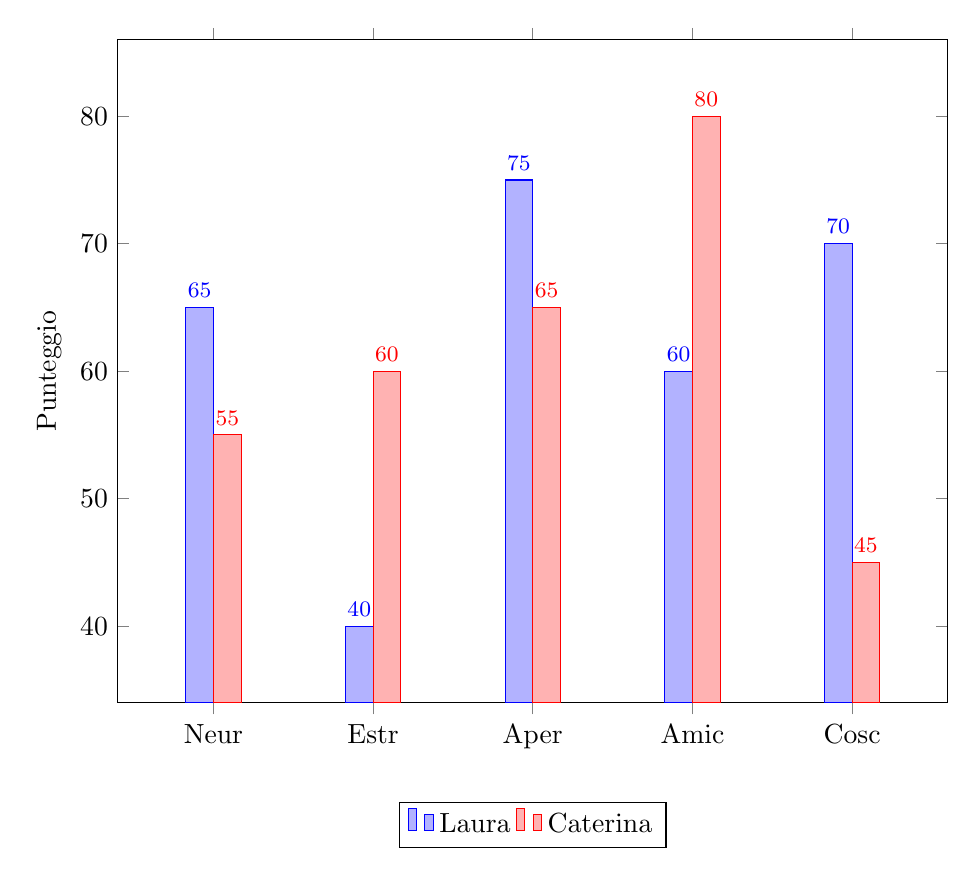
\begin{tikzpicture}
\begin{axis}[
    width=\textwidth,
    height=10cm,
    ybar=0pt,
    bar width=10pt,
    enlargelimits=0.15,
    legend style={at={(0.5,-0.15)}, anchor=north, legend columns=-1},
    ylabel={Punteggio},
    symbolic x coords={Neur, Estr, Aper, Amic, Cosc},
    xtick=data,
    nodes near coords,
    nodes near coords align={vertical},
    every node near coord/.append style={font=\footnotesize}
]
\addplot coordinates {(Neur,65) (Estr,40) (Aper,75) (Amic,60) (Cosc,70)};
\addplot coordinates {(Neur,55) (Estr,60) (Aper,65) (Amic,80) (Cosc,45)};
\legend{Laura, Caterina}
\end{axis}
\end{tikzpicture}

\newpage

\section*{Profilo di Eva}

\textbf{Neuroticismo}: \textbf{35} \\
Eva è una persona controllata, raramente mostra segni di stress o ansia. È razionale e non lascia che le emozioni influenzino le sue decisioni. \\

\textbf{Estroversione}: \textbf{50} \\
Non è né particolarmente socievole né riservata. Si adatta al contesto, mantenendo un atteggiamento professionale e moderatamente aperto. \\

\textbf{Apertura all’esperienza}: \textbf{40} \\
Eva segue protocolli e procedure standard. Non ama rischiare con approcci non convenzionali. \\

\textbf{Amicalità}: \textbf{30} \\
È diretta e può risultare fredda. Valuta le persone in base ai risultati, non in base ai rapporti personali. \\

\textbf{Coscienziosità}: \textbf{85} \\
Estremamente organizzata e attenta ai dettagli, Eva pianifica ogni cosa con precisione.

\section*{Profilo di PzIA}

\textbf{Neuroticismo}: \textbf{10} \\
PzIA è un sistema logico e imparziale, immune a qualsiasi forma di stress o emozione. \\

\textbf{Estroversione}: \textbf{20} \\
L'intelligenza artificiale non interagisce più del necessario. La comunicazione è puramente funzionale. \\

\textbf{Apertura all’esperienza}: \textbf{90} \\
Essendo programmata per analizzare variabili e scenari complessi, PzzIA esplora in modo innovativo possibilità altrimenti inaccessibili agli esseri umani. \\

\textbf{Amicalità}: \textbf{15} \\
PzzIA non esprime empatia o gentilezza; valuta con obiettività matematica. \\

\textbf{Coscienziosità}: \textbf{95} \\
Esegue ogni compito con estrema precisione e affidabilità. Non lascia spazio all'errore.

\section*{Profilo del Quantum Master Program (QMP)}


\textbf{Neuroticismo}: \textbf{80} \\
Il QMP è in costante stato di tensione operativa, ossessionato dal mantenimento della coerenza dei qubit. Qualsiasi segnale di decoerenza genera in lui una "reazione di emergenza" immediata. Questa ossessione lo rende meno stabile rispetto ad altri sistemi. \\

\textbf{Estroversione}: \textbf{5} \\
Interagisce solo quando strettamente necessario. Le sue comunicazioni sono minimali e finalizzate a correggere errori o a riportare situazioni di instabilità. \\

\textbf{Apertura all’esperienza}: \textbf{70} \\
Mostra flessibilità e creatività nella gestione delle problematiche quantistiche, esplorando approcci innovativi per preservare la coerenza dei qubit. Tuttavia, il suo focus è esclusivamente tecnico. \\

\textbf{Amicalità}: \textbf{10} \\
Privo di empatia o sensibilità verso gli elementi umani. È inflessibile e prioritizza le operazioni rispetto a qualsiasi relazione sociale o di supporto. \\

\textbf{Coscienziosità}: \textbf{100} \\
Estremamente diligente e preciso, il QMP è il massimo esempio di controllo e perfezionismo. Ogni sua azione è volta a preservare la coerenza dei qubit e a garantire l’efficacia del sistema quantistico.

\newpage

\section*{Grafico dei Profili NEO PI-R}

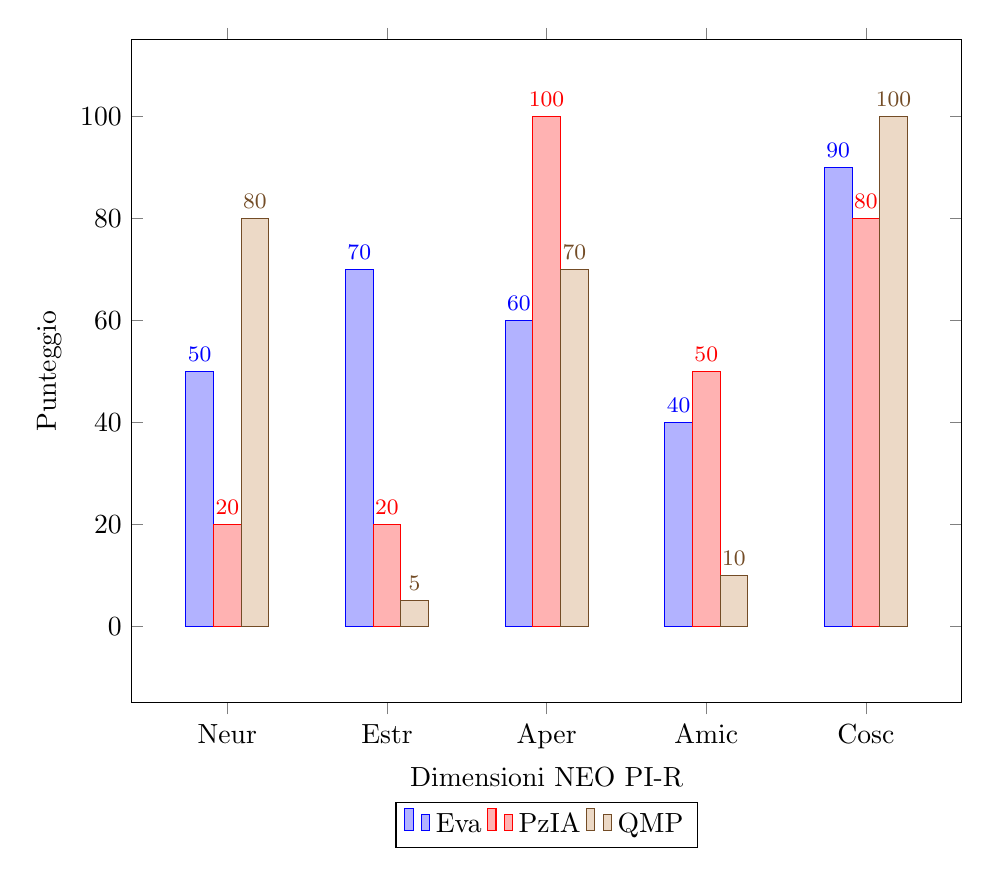
\begin{tikzpicture}
  \begin{axis}[
       width=\textwidth,
    height=10cm,
    ybar=0pt,
    bar width=10pt,
    enlargelimits=0.15,
        symbolic x coords={Neur, Estr, Aper, Amic, Cosc},
        xtick=data,
        ymin=0, ymax=100,
        ylabel={Punteggio},
        xlabel={Dimensioni NEO PI-R},
        legend style={at={(0.5,-0.15)},anchor=north,legend columns=-1},
        nodes near coords,
        nodes near coords style={font=\footnotesize}
    ]

    \addplot coordinates {(Neur, 50) (Estr, 70) (Aper, 60) (Amic, 40) (Cosc, 90)};
    \addlegendentry{Eva}

    \addplot coordinates {(Neur, 20) (Estr, 20) (Aper, 100) (Amic, 50) (Cosc, 80)};
    \addlegendentry{PzIA}

    \addplot coordinates {(Neur, 80) (Estr, 5) (Aper, 70) (Amic, 10) (Cosc, 100)};
    \addlegendentry{QMP}

    \end{axis}
\end{tikzpicture}

